%\documentclass[12pt]{scrreprt}
\documentclass[12pt]{report} 

% language may be romanian or english (default is english)
% type may be bachelor or master (default is bachelor)
\usepackage[language=english, type=bachelor]{style}
\usepackage{amsmath}
\usepackage{adjustbox}


%\geometry{a4paper,top=2.5cm,left=3cm,right=2.5cm,bottom=2.5cm}
%in style
%controlling the appearance of your headers and footers
\usepackage{fancyhdr}
\pagestyle{fancy}
\lhead{}
\chead{}
\renewcommand{\headrulewidth}{0.2pt}
\renewcommand{\footrulewidth}{0.2pt}

\begin{document}

\specialization{COMPUTER SCIENCE ROMANIAN}	
\title{Depression signs detection}					   
\author{Dinică Mircea}											
\supervisor{Lect. PhD. Lupea Mihaiela}				
				
\maketitle


\newpage
\thispagestyle{empty}
\mbox{}
\newpage
\pagenumbering{roman} 

\cleardoublepage
ABSTRACT
\vspace{0.5cm}	
\hrule
\vspace{0.5cm}	
%\cleardoublepage

The purpose of this paper is to develop Artifical Intelligence (AI) classifiers that detect if the text shows signs of depression or not in two languages: English and Romanian. Depression is a major problem right now, which if not addressed can cause serious problems. With the help of NLP and AI, it is desired to develop a tool for giving an opportunity to its users to have an easy way to get an initial assessment of their texts, in cases such as private text messages, their own thoughts or even help professionals reach possible clients in order to help them. 

The two classifiers will be created using the same dataset for training. The model that processes English text will use the original dataset in English. For the Romanian model, the dataset is translated using a Python library with the Google Translate API. For pre-processing, a tool called Linguistic Inquiry and Word Count will be used. The English model will use the latest version, LIWC-22, developed in 2022. The Romanian model will use the most recent translated version, LIWC-2015, developed in 2015. Both classifiers will use the Random Forest model.

As a practical tool for the algorithm, a chrome extension which expects as input a text was developed. The output is the class which the model predicted with a corresponding message advising the user to investigate further with the author of the text. This will be computed on a web back-end server, where the AI classifier is used, respecting the REST architectural style. The chosen technologies for developing the tool are Python with Flask framework for the back-end server and React, the JavaScript library for the front-end server.

The application can work in multiple languages because it uses the same Python library that was used to translate the dataset. The input text is translated when the language it is written in is different from Romanian or English.  

\tableofcontents


\newpage
\pagenumbering{arabic}

\chapter{Introduction}

%\chapter*{Introduction}
\label{intro}

% \par Introducere: obiectivele lucrarii si descrierea succinta a capitolelor, prezentarea temei, prezentarea contributiei proprii, respectiv a rezultatelor originale si mentionarea (daca este cazul) a sesiunii de comunicari unde a fost prezentata sau a revistei unde a fost publicata.
%THEME PRESENTATION
\section{Depression Statistics and Insights}
\label{sec:ch1sec1}

\par \quad Depression stands as a mental health affliction with profound impacts on both psychological and physical well-being. Characterized by a disinterest in routine activities, sleep disturbances, anhedonia, and in severe cases, suicidal ideation \cite{cui2015systematic}, it has become a problem across worldwide. Furthermore, individuals with major depressive disorder face a bigger risk of cardiovascular problems, not optimal treatment outcomes, and higher rates of morbidity and mortality \cite{seligman2015interface,luo2018effects}.

The World Health Organization (WHO) identifies depression as the primary contributor to global disability, affecting over 300 million individuals worldwide \cite{smith2014world}. Particularly alarming is the revelation that adolescents with severe depression are 30 times more prone to suicide \cite{stringaris2017depression}. 
Although we know depression is a big problem worldwide, we still don't fully understand what causes it. We know that cultural, psychological, and biological factors play a part, but we don't know exactly how they all fit together.\cite{gross2014silver,menard2016pathogenesis}.

The Global Burden of Disease (GBD) study \cite{liu2020changes} offers comprehensive insights into various mental problems across 195 countries, including depression. Divided into dysthymia and major depressive disorder categories, the GBD database from 1990 to 2017 furnishes valuable data for understanding depression's evolution globally. Major depressive disorder emerges as a predominant form of depression, posing a significant burden on global health, indicating it may become the leading cause of disability by 2030. Moreover, while dysthymia rates decreased in some regions, it remains a concern, particularly in the United States.

Identifying underlying causes and risk factors for depression, including genetic predisposition, demographic factors, unhealthy lifestyles, and diseases coming from it such as stroke, cancer, and AIDS, highlights the need for a change. Governments in countries with high depression rates are encouraged to prioritize research, promote healthy lifestyles, and ensure comprehensive care for individuals with predisposing conditions. However, the study acknowledges limitations in data analysis, advocating for future research of regional risk factors and guide tailored policy interventions for effective depression control globally. This can be seen in Figure \ref{FigGloablDepression} \cite{liu2020changes}, which evaluated the worldwide burden of depression using the estimated annual percentage change (EAPC) and age-standardized incidence rate (ASR).

\begin{figure}[htbp]
	\centering
		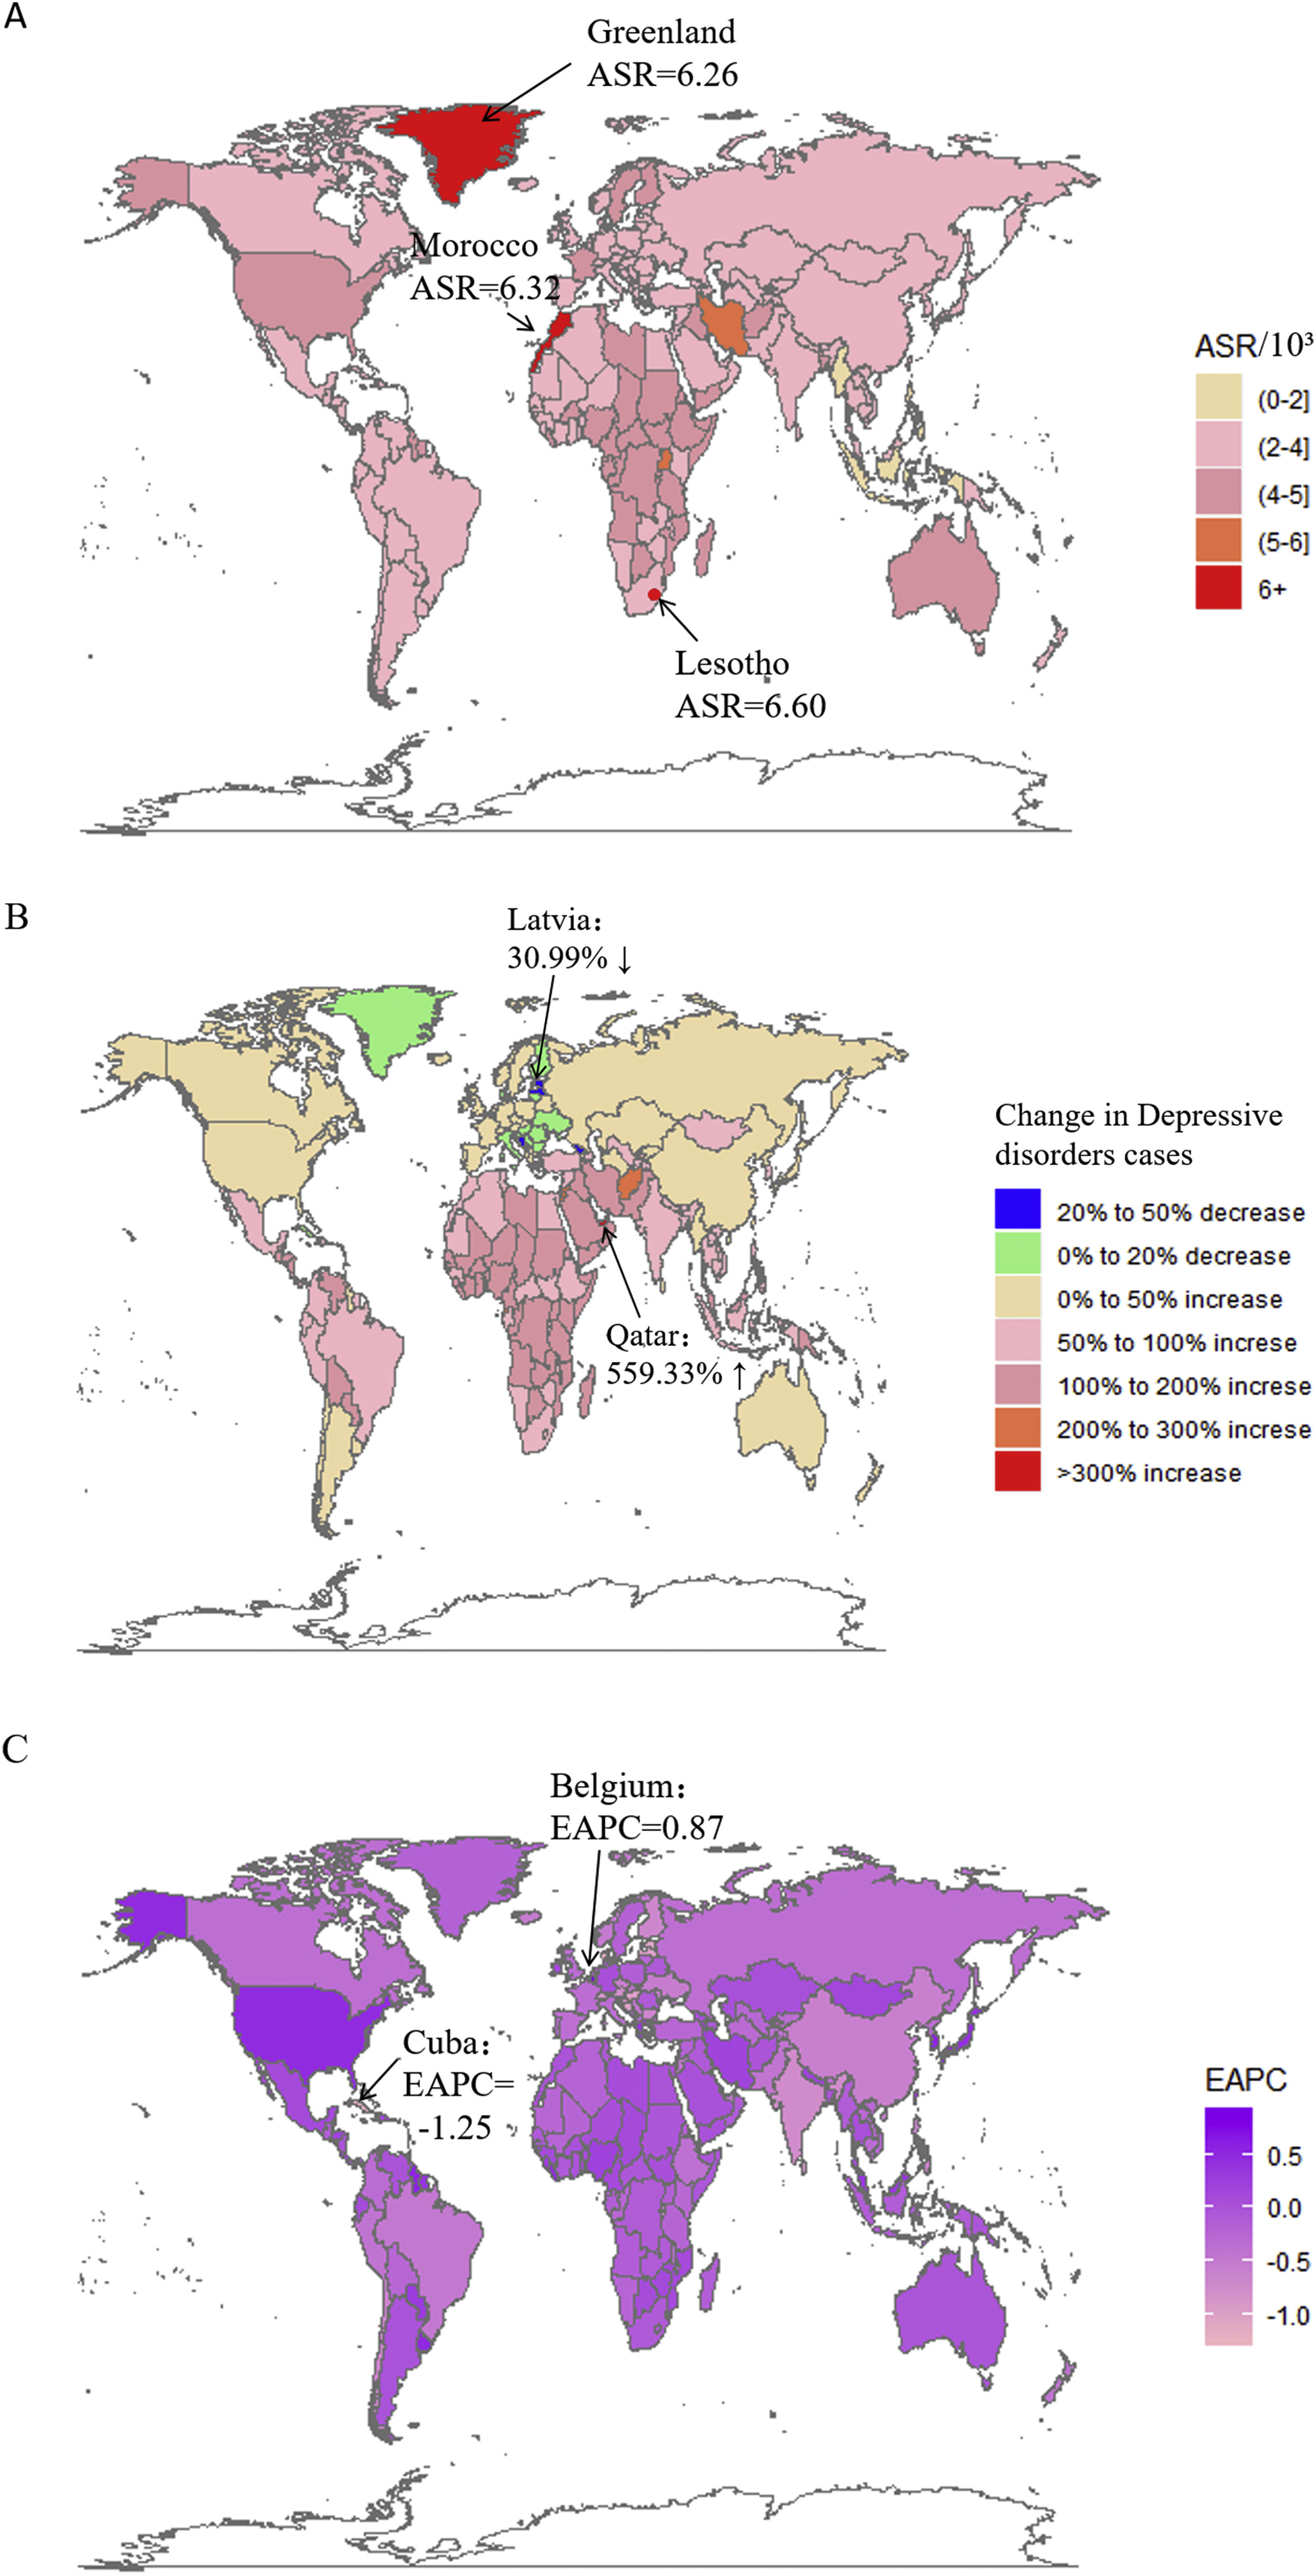
\includegraphics[scale=0.65]{./figures/depression-map-Liu-et-al-2020.jpg}
	\caption{Global depression statistics comparison between 1990 and 2017 \cite{liu2020changes}}
	\label{FigGloablDepression}
\end{figure}

\section{Problem Statement}
\quad As discussed in the previous section, depression is a mental health condition that significantly affects both mind and body. It often involves losing interest in daily activities, having trouble sleeping, not being able to feel joy, and in severe cases, experiencing suicidal thoughts. People with major depression also face higher risks of heart problems, poor treatment results, and increased rates of sickness and death.

This highlights the importance of preventing depression on a global scale. To achieve this, it is essential to create a tool that can detect and address depression in various languages. Such a tool would help people from different linguistic backgrounds receive the support they need.


\section{Related Work}

\quad The field of computer science dedicated to processing text data, known as Natural Language Processing (NLP), originated in the 1950s with the Georgetown Experiment \cite{hutchins2004georgetown}, which involved automatic translation from Russian to English. Numerous NLP tasks such as machine translation, document summarization, part-of-speech tagging, named-entity recognition, and sentiment analysis have been effectively addressed to date. The techniques developed have been incorporated into many cutting-edge applications. 

Concerning binary classification for depression, another explored method was the utilization of smartphone behavioral indicators \cite{opoku2021predicting}. Employing five supervised machine learning algorithms: random forest (RF), support vector machine (SVM) with a radial basis function (RBF) kernel, and XGBoost (XGB), it attained the following performance metrics: recall between 85.55\% and 92.51\%; F1 score from 92.19\% to 95.56\%; area under receiver operating characteristic curve ranging from 88.73\% to 94.00\%; Cohen's kappa between 94.69\% and 99.06\%; and accuracy scores from 86.61\% to 92.90\%, with 96.44\% to 98.14\%.

As for the training of ML models with multi-lingual data, another research detailed the outcomes of training identical models on the original IMDB movie review dataset in English, alongside three other datasets translated into German, Hindi, and Urdu using Google Translate \cite{ghafoor2021impact}. The most accurate results in English were obtained by the support vector machine, achieving 90.45\% accuracy. For the other languages, the accuracies were 90.01\% in German, 87.26\% in Urdu, and 82.30\% in Hindi. This indicates that while translation may serve as an effective method for data acquisition in some languages, it may only be moderately successful in others.


A further investigation discussed the previously mentioned issue of translating datasets for languages with less scientific research done for, focusing on email spam detection in Urdu \cite{siddique2021machine}. The dataset, originally in English, was translated using the googletrans library \cite{googletranslib}, and training was conducted with two machine learning algorithms: support vector machine (SVM) and Naive Bayes, as well as two deep learning architectures: long short-term memory networks (LSTM) and convolutional neural networks (CNN). The models demonstrated accuracies as follows: LSTM achieved 98.4\%, CNN recorded 96.2\%, Naive Bayes reached 98.0\%, and SVM obtained 97.5\%.

\section{Objective}
\label{sec:ch1sec2}

\quad The objective of this scientific study is to leverage machine learning techniques to develop a tool for identifying depression through textual analysis. By using natural language processing (NLP) and artificial intelligence (AI), the goal is to create a tool capable of detecting signs of depression in text-based communications.

The purpose is to achieve two main objectives:
\begin{itemize}
     
\item \textbf{Objective 1}: Provide an accessible application of identifying individuals who may be experiencing symptoms of depression. By analyzing the language used in written communications, such as social media posts, emails, or chat messages, the tool aims to offer an initial assessment of an individual's mental well-being. This approach can facilitate early intervention and support, potentially preventing more severe depressive symptoms and their associated consequences.

\item \textbf{Objective 2}: Evaluate the performance of the machine learning model in a cross-linguistic context. To achieve this, the English dataset will be translated to Romanian and assess the performance of the model on both language versions. This comparative analysis will tell if the tool is accurate across different languages and cultural contexts.

\end{itemize}

With this study the hope is to contribute to the advancement of computational techniques for mental health assessment and also expand the research available for the Romanian language. The aim is to provide clinicians, researchers, and individuals themselves with a valuable resource for early detection and prevention of depression, ultimately encouraging improved mental well-being and quality of life.


\section{Paper Structure}

\quad This paper describes its content in six chapters. Chapter 1 provides the motivation  purpose of the depression detection application. Chapter 2 
covers the key theoretical concepts that form the basic ideas on which the application is built. Chapter 3 gives details regarding the dataset used and its translation into Romanian Language and the pre-processing techniques, namely Linguistic Word Inquiry and Word Count which recognizes the emotions and grammar parts which the tokens belong to. Chapter 4 describes why the machine learning classification algorithm Random Forest was chosen, and also the results of the three training experiments, two on the English original dataset and one on the translated dataset in Romanian. 
Chapter 5 summarizes the architecture and technologies used to implement the practical tool. The final chapter outlines the conclusions and proposes future development ideas. 
%\addcontentsline{toc}{chapter}{Introducere}
%\addcontentsline{toc}{chapter}{Introduction}

\chapter{Theoretical Background}

\label{chap:ch2}
\section{Natural Language Processing}

\quad This section explores Natural Language Processing (NLP), an important area in artificial intelligence that focuses on how computers understand and work with human language. NLP combines language studies with machine learning techniques to help machines understand, interpret, and generate human language in a useful way.

The basics of NLP are built on various tasks that address different parts of language processing. These tasks range from simple text handling to more complex activities like translating languages, analyzing emotions in text, and identifying important entities such as names and dates. By looking at these common NLP tasks, this section aims to provide an overview of the most common methods and algorithms that enable machines to process natural language.

\textbf{Tokenization} is the process of splitting text into individual words or tokens. This is a fundamental step for many NLP tasks, as it breaks down the text into manageable pieces that can be analyzed separately. Proper tokenization is crucial because it directly affects the performance of subsequent NLP processes. Challenges in tokenization include handling punctuation, contractions, and different languages.

\textbf{Part-of-speech tagging} involves labeling each word in a text with its corresponding part of speech, such as noun, verb, adjective, etc. This task helps in understanding the grammatical structure of sentences, providing valuable information about word relationships and functions. Accurate part-of-speech tagging is essential for more advanced NLP tasks like parsing and semantic analysis. The complexity arises from the fact that many words can serve multiple grammatical roles depending on the context.

\textbf{Named Entity Recognition} (NER) is the process of identifying and categorizing entities such as names, dates, and organizations within a text. This task is crucial for extracting structured information from unstructured text, enabling applications like information retrieval, question answering, and content recommendation. NER systems must be able to handle the ambiguity and variability of language, as entities can often be represented in numerous ways.

\textbf{Sentiment analysis} aims to determine the emotional tone behind a series of words, making it a powerful tool for understanding opinions and attitudes expressed in text. This task is commonly used in social media monitoring, customer feedback analysis, and market research. Sentiment analysis can be challenging due to the particularities of human emotion, sarcasm, and context-specific sentiment expressions.

\textbf{Machine translation} involves converting text from one language to another. This task requires a deep understanding of both the source and target languages, including their syntax, semantics, and cultural subtleties. Effective machine translation systems use sophisticated algorithms and large parallel corpora to produce accurate and fluent translations. Despite significant advancements, machine translation still faces challenges like idiomatic expressions, context preservation, and handling low-resource languages.

\textbf{Text summarization} aims to create a summary of a longer document, enabling quick understanding of the main points. This task can be performed through extractive methods, which select key sentences from the original text, or abstractive methods, which generate new sentences that capture the essence of the original content. Text summarization is useful in various applications, including news aggregation, academic research, and content curation.

Each of these tasks plays a crucial role in enabling machines to understand and process human language, highlighting the diverse and complex nature of NLP.

\section{Machine Learning Algorithms in Classification}

Machine learning algorithms play a key role in classification tasks, helping us to categorize data into different groups. This section will explore various algorithms commonly used for classification while looking at a comprehensive study that evaluated twelve distinct machine learning algorithms across seven datasets \cite{siraj2023performanceModelComparison}.

The study \cite{siraj2023performanceModelComparison} in question compared the performance of several algorithms, including Naive Bayes (NB), Linear Discriminant Analysis (LDA), Logistic Regression (LR), Artificial Neural Networks (ANN), Support Vector Machines (SVM), K-Nearest Neighbors (K-NN), Hoeffding Tree (HT), Decision Tree (DT), C4.5, Classification and Regression Tree (CART), Random Forest (RF), and Bayesian Belief Networks (BB), across multiple metrics. Among these, Random Forest showed the most consistent and high results, showing superior accuracy, precision, and Matthew’s Correlation Coefficient (MCC). Following Random Forest, the algorithms of Neural Networks (NN), Naive Bayes (NB), Bayesian Belief Networks (BB), and Logistic Regression (LR) were identified as the next most effective, in descending order of accuracy.

The study \cite{siraj2023performanceModelComparison} also highlighted the significance of the kappa statistic and Root Mean Square Error (RMSE) as important factors in assessing model performance, further validating the consistency of Random Forest in handling diverse and complex datasets. With these statistics, and in accordance with the study’s conclusion, the selection of Random Forest is motivated by its results across multiple validation metrics.

The datasets utilized for the comparative study are varied, each with its unique characteristics and relevance to different classification tasks:
\begin{itemize}
 
\item Breast Cancer Wisconsin (Original): This dataset contains 11 attributes and is used for binary classification (two classes) with 699 instances. It does include missing values, which would require additional preprocessing steps.

\item Statlog (Vehicle Silhouettes): Comprising 19 attributes over 846 instances, this dataset is for multiclass classification with four distinct classes and has no missing values.

\item Vertebral Column: With 7 attributes and 310 instances, this dataset is also used for multiclass classification, distinguishing among three classes, without any missing values.

\item Breast Tissue: This dataset has 10 attributes across 106 instances and is used for a more complex multiclass classification task with six classes, also free of missing values.

\item Contraceptive Method Choice: It includes 10 attributes and a larger number of instances at 1473. It’s structured for multiclass classification into three classes, and there are no missing values.

\item Image Segmentation: This is a sizable dataset with 20 attributes and 2310 instances for multiclass classification involving seven classes, and it contains no missing values.

\item Artificial Characters: The largest among the datasets listed, it boasts 8 attributes across a substantial 10218 instances. It’s designed for a multiclass classification with ten classes, and like most others here, it lacks missing values.

\end{itemize}

Across the datasets analyzed in the study \cite{siraj2023performanceModelComparison}, Random Forest (RF) consistently was one of the best algorithms. Its F-measure and Matthew's Correlation Coefficient (MCC) values were notably high, often outperforming other algorithms. For instance, RF attained an accuracy of 98.48\%, kappa value of 98.23\%, and precision and recall rates both at 98.5\% on certain datasets, alongside a specificity of up to 99.7%.

While K-NN and Logistic Regression (LR) also demonstrated strong performances in certain cases, with K-NN leading in precision and recall in the Breast Tissue dataset and LR excelling with the highest MCC values for the Vehicle and Vertebral Column datasets, RF's overall dominance was clear. RF's ability to achieve the lowest error rates, coupled with the lowest root mean square error in the majority of datasets, further confirms its reliability as an algorithm for complex predictive tasks, including depression detection.

\section{Random Forest}

\quad The Random Forest algorithm is a popular machine learning method used for both classification and regression tasks. It is known for its simplicity, flexibility, and strong performance on a wide range of problems. This section provides a general overview of how Random Forest works and why it is widely used in the field of machine learning.

At its core, Random Forest is an ensemble learning technique. This means it builds multiple models and combines their results to improve overall performance. Specifically, Random Forest creates a large number of decision trees during training time and merges their outputs to make a final prediction. Each decision tree is trained on a different subset of the training data, which is chosen randomly. This process is known as bootstrapping.

A decision tree works like a flowchart, where each decision point (node) asks a question about the value of a feature, and the answer leads to another question or a final decision (leaf). At the top of the tree is the root node, which represents the first question. Based on the answer, the data moves down the tree to the next node. This process continues until a leaf node is reached, which gives the prediction or outcome, as seen in Figure \ref{randomForestVisualized}.

\begin{figure}[htbp]
	\centering
		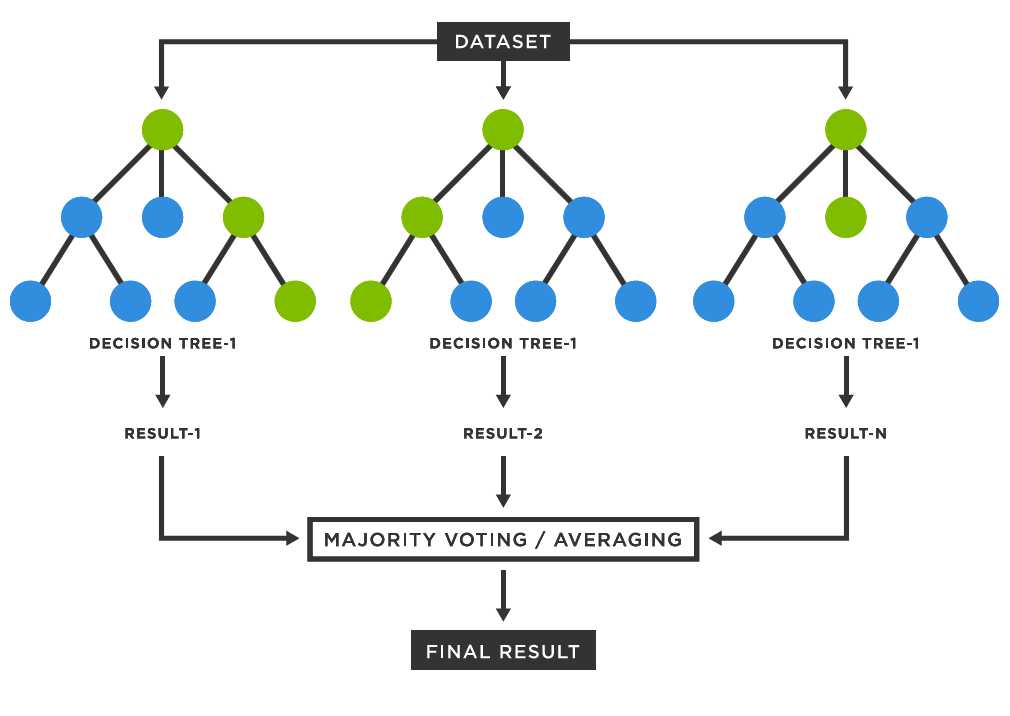
\includegraphics[scale=0.4]{LaTeX Bachelor Thesis Depression Signs Detection/figures/RandomForestVisualized.png}
        \caption{Random Forest Visualized \cite{predikdata2023}}
	\label{randomForestVisualized}
\end{figure}

One of the key features of Random Forest is that it introduces randomness not only in the selection of data samples but also in the selection of features used to split nodes in the trees. This randomness helps in making the model less likely to overfit the training data. Overfitting occurs when a model learns the training data too well, including its noise and outliers, and performs poorly on new, unseen data.

In classification tasks, each decision tree in the forest votes for a class, and the class with the most votes is chosen as the final prediction. In regression tasks, the average of the outputs from all trees is taken as the final result. This ensemble approach generally leads to higher accuracy and better generalization compared to using a single decision tree.

Random Forest has several advantages. It is easy to use and tune, often requiring fewer parameters compared to other complex algorithms. It handles large datasets with higher dimensionality well and maintains good performance even when a large proportion of the data is missing. Additionally, it can give insights into the importance of different features in the data, which can be useful for understanding underlying patterns.

However, Random Forest also has some limitations. It can be computationally expensive and slow to train when dealing with a large number of trees or very large datasets. The model can also become less interpretable as the number of trees increases, making it harder to understand the decision-making process compared to a single decision tree.

\section{Evaluation Metrics}
\quad Metrics are a crucial part of evaluating the effectiveness of a binary classifier. It's important to use a variety of tools and methods to understand different aspects of the model's performance. Here the metrics that were chosen for the evaluation of the depression binary classifier:

\begin{itemize}
     \item \textbf{Confusion Matrix}: This is a table that visualizes the performance of the binary classifier by showing the actual versus predicted classifications. The matrix contains the values: TP (true positives), TN (true negatives), FP (false positives), and FN (false negatives). It helps identify the kinds of errors the model is making, such as confusing one class for another.
     
    \item \textbf{Classification Metrics}: These include accuracy, precision, recall, and the F1-score, which together provide a comprehensive overview of overall model performance. 
    \begin{itemize}
        \item \textbf{Accuracy} measures the overall correctness of the model across all predictions (formula \ref{accuracy}). 
        \item \textbf{Precision} assesses how many of the positively predicted cases were actually positive 
 (formula \ref{precision}).
        \item \textbf{Recall} (or sensitivity) determines how many of the actual positive cases were correctly identified by the model (formula \ref{recall}).
        \item \textbf{F1-Score} is the harmonic mean of precision and recall, helping balance the two in scenarios where one may be more important than the other 
 (formula \ref{f1}).
        
        \begin{align} 
            &\mathit{Accuracy} = \frac{TP+TN}{TP+TN+FP+FN} \label{accuracy}\\
            &\mathit{Precision} = \frac{TP}{TP+FP} \label{precision}\\
            &\mathit{Recall} = \frac{TP}{TP+FN} \label{recall}\\
            &F1-Score = \frac{2*\mathit{Precision}*\mathit{Recall}}{\mathit{Precision}+\mathit{Recall} \label{f1}}
        \end{align}
    \end{itemize}
       \item \textbf{ROC Curve}: This graph shows the ability of the model to distinguish between the two classes at various threshold levels. It plots the true positive rate against the false positive rate, providing insight into the trade-offs between capturing positives and avoiding false alarms \cite{hoo2017roc}.
    \item \textbf{Feature Importance}: This metric highlights which features (variables) in your data have the most influence on the model’s predictions. Understanding feature importance can help in refining the model by focusing on the most relevant factors.
\end{itemize}

By using these metrics, a detailed understanding of your model's strengths and weaknesses can be achieved, guiding improvements and ensuring it performs well across various conditions.
%\chapter{Dataset Analysis and Pre-processing Techniques}
\chapter{Dataset and LIWC}

\label{chap:ch3}

\par
\section{Dataset Overview}

\quad Our AI model relies on a dataset \cite{depressionDataset}, crafted in order to advance in mental health classification research. Gathered through web scraping techniques from diverse Subreddits, this dataset contains discussions and viewpoints on mental health topics. The aim of creating this dataset was to examine textual patterns which indicate depression's presence or absence in individuals, as seen from their online conversations .

% \subsection{Collection Methodology}
The raw data was sourced by employing web scraping techniques, targeting specific Subreddits known for their discussions on mental health issues. This approach ensured that the data collected was relevant to the research objectives, capturing a diverse range of experiences and expressions related to mental health.

% \subsection{Dataset Overview}
Comprising 7,650 unique entries, the dataset is enough for an accurate machine learning algorithm. Each entry is annotated with an is\textunderscore depression label, distinguishing between texts that indicate the presence of depression (labeled '1') and those that do not (labeled '0'). This labeling process was carried out with careful consideration to ensure accuracy and reliability in the classification \cite{depressionDataset}.

A noteworthy aspect of the dataset is its well-balanced nature, with 3,900 entries labeled as non-depression and 3,831 entries indicating depression. This balance is important in avoiding bias in the predictive modeling process, ensuring that the resulting classification model is accurate.

Also the raw data underwent a cleaning process using multiple Natural Language Processing (NLP) techniques. This prep-rocessing phase was crucial for eliminating noise, such as irrelevant characters, web links, and non-English words, thereby refining the dataset for analysis. The cleaning process also involved normalizing the text to ensure consistency across the dataset, facilitating more effective data analysis and model training \cite{depressionDataset}.

\subsection{Dataset Translation for Romanian Language}
\par \quad Multilingual depression detection is highly dependant on the capability of AI models to understand and analyze text from different cultures. This section describes the process of translating English text into Romanian, a step essential for training our AI model to recognize depressive patterns in a multilingual context. We will discuss the selection criteria and the impact of utilizing a specific Translation API to bridge the language gap, thus enabling our model to process and interpret Romanian text with the same level of accuracy as English. 

\subsection{Reasoning Behind Choosing Yandex}

\quad In our effort to refine our multilingual depression detection model, we referenced a detailed study that assessed the efficiency, accuracy, and security of various Translation APIs \cite{rashmi2020comparison}. This comparative analysis served as the foundation for selecting the most suitable API for our application, which required the translation of text from English to Romanian among other language pairs. The study meticulously compared several leading Translation APIs, including Google API, Microsoft, Systran.io, MyMemory, and Yandex, focusing on their performance in terms of speed, accuracy, security, and the breadth of language support.
\begin{itemize}
\item \textbf{Google API} is widely recognized for its impressive language support, capable of translating content across more than 100 languages. This extensive reach makes it a versatile tool for global communication and content translation. Its reputation and prevalence in the market are testaments to its utility and user-friendly interface. Additionally, it's worth noting that while Google API is commendable, it is not a free service, which may affect its accessibility for some users.\cite{rashmi2020comparison}.

\item \textbf{Microsoft's Translation API} is lauded for its quality and security, offering translations among 60+ languages. It stands out for its emphasis on accuracy and stringent security protocols, although its language support is less extensive than Google's \cite{rashmi2020comparison}.

\item \textbf{Systran.io} boasts a high accuracy rate of 99\%, albeit with limitations in recognizing slang, nuances, and culturally relevant phrases. Its security is commendable, positioning it as a reliable choice for many applications \cite{rashmi2020comparison}.

\item \textbf{MyMemory} excels in translation speed but experiences the highest latency among the APIs evaluated. While it supports translations between 80+ languages, the absence of training data for certain language combinations limits its effectiveness. Nonetheless, its security is robust \cite{rashmi2020comparison}.

\item \textbf{Yandex API}, with support for 90+ languages, stands out for its balance of translation accuracy and lower latency compared to its counterparts. Despite its efficiency and broad language coverage, its security features are not optimal for translating confidential documents \cite{rashmi2020comparison}.
\end{itemize}

The conclusion from this study discussed the strengths and weaknesses of each API, guiding our choice towards Yandex API for our multilingual depression detection model. Yandex was selected due to its free access, lower latency, and reliable accuracy across different cultures, making it an ideal tool for everyday translations where security is not the biggest concern \cite{rashmi2020comparison}. This choice aligns with our objective of giving people an easy to use and accessible tool in order to prevent problems that could appear with depression.

Another rigorous study \cite{cambedda2021study} provides a nuanced error analysis of Yandex's translations. Notably, Yandex's performance, depicted in the graph \ref{YandexTranslationPerformance}, indicates a relatively uniform distribution of errors across multiple categories. This suggests that while Yandex does have areas where it lacks consitency, such as Lexis, Syntax, and Article Usage, it generally maintains the core meaning of the translated text. This is critical for our model, which relies on emotion categories to accurately detect depression in text.

\begin{figure}[htbp]
	\centering
		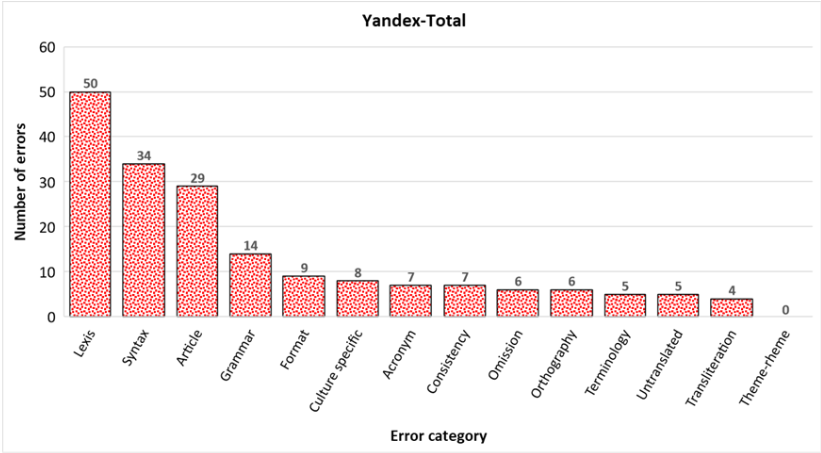
\includegraphics[scale=0.65]{LaTeX Bachelor Thesis Depression Signs Detection/figures/Yandex's-translation-performace.png}
	\caption{Yandex's translation performance \cite{cambedda2021study}}
	\label{YandexTranslationPerformance}
\end{figure}

The Lexis category, in particular, displays the highest number of errors, signaling a need for further investigation to understand whether these issues are from the nature of the texts or from challenges within the translation tool. However, it is encouraging to note that error categories such as Grammar, Format, Culture-Specific References, Acronym, and Consistency show significantly fewer errors. These categories are essential for maintaining the general meaning, which reaffirms our choice of Yandex for texts where nuanced meaning is less likely to affect the detection of depression signs.

Further examination of the study indicates that Yandex demonstrates a more adept handling of common language texts as opposed to those with specialized jargon, registering fewer errors in translations of texts with language spoken by the people in a particular country or region \cite{cambedda2021study}. Considering our dataset comprises of Reddit posts, which are typically phrased in everyday language, this finding is particularly relevant. The study also highlights that, with the exception of Article Usage, the disparity in error rates between different text types is negligible, suggesting that Yandex can reliably manage the conversational and informal style characteristic of Reddit communications.

\subsection{Adjusting to Yandex API's Policy Shift}

\quad We had initially recognized the Yandex API as a superior option, particularly for its cost-effectiveness, as it was freely accessible at the time of study \cite{rashmi2020comparison}. This advantage aligned with our objectives, allowing us to use its translation capabilities without financial constraints.

However, since the publication of \cite{rashmi2020comparison}, Yandex's policy has undergone significant changes. The API, once free to use within a given generous limit, now requires users to possess a registered and legally recognized company to utilize its services. Ihe requirement of company registration introduces a barrier, limiting the accessibility of Yandex API for independent researchers, small teams, or educational institutions.

Given these new rules, we are still fully dedicated to creating a useful and easy-to-use depression detection system that works in many languages. Therefore, we are looking into different approaches.

\subsection{Shifting to googletrans}

\quad We decided to integrate the googletrans library \cite{googletranslib} into our multilingual depression detection model. It offers a free and unlimited Python library that uses the Google Translate API. This library appears particularly advantageous for our requirements, as it is not only accessible without cost but also does not require the a company registration that Yandex now demands. As it can be seen in \ref{codeGoogleTransUsage}, it is very accessible to translate text in Python from English ro Romanian.

\begin{figure}[htbp]
	\centering
		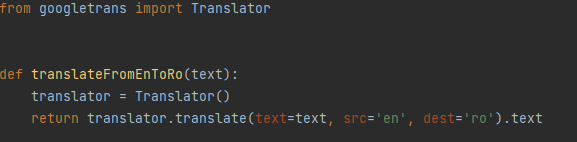
\includegraphics[scale=1]{LaTeX Bachelor Thesis Depression Signs Detection/figures/codeGoogleTransUsage.png}
	\caption{Python library "googletrans" translation from English to Romanian}
	\label{codeGoogleTransUsage}
\end{figure}

The googletrans library \cite{googletranslib} has features that are well-suited to our project's needs. It is recognized for its speed and reliability, as it operates on the same servers as translate.google.com. The library supports auto language detection, facilitating the identification and translation of a wide array of languages without prior specification. Additionally, it provides the capability for bulk translations, which is invaluable when processing large datasets typically found in NLP tasks. It was done for the chosen dataset \cite{depressionDataset} in Python as it can be seen in \ref{codeDatasetTranslation} .

\begin{figure}[htbp]
	\centering
		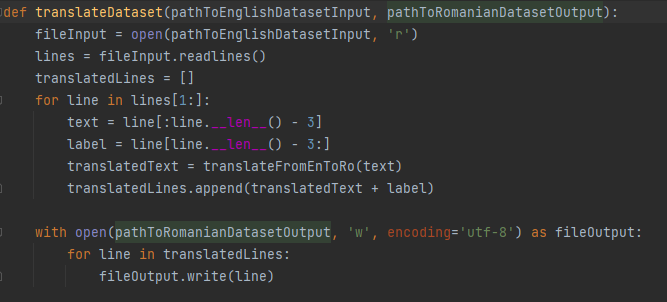
\includegraphics[scale=1]{LaTeX Bachelor Thesis Depression Signs Detection/figures/codeDatasetTranslation.png}
	\caption{Python code for translating dataset from English to Romanian}
	\label{codeDatasetTranslation}
\end{figure}

It is also important to acknowledge googletrans's \cite{googletranslib} usage notes. The 15,000-character limit per text may require segmentation of longer entries, and the instability of web-based translation services means that we should proceed with precaution regarding the library's reliability. The developers themselves suggest opting for the official Google Translate API for more advanced applications where stability is very important. Furthermore, potential HTTP errors could indicate temporary bans by Google, meaning that it is needed to keep an eye on and manage how we use our API to avoid any interruptions. Despite these considerations, the googletrans library's free and flexible usage makes it an excellent fit for our project in its current stage.


\section{Leveraging LIWC for Textual Analysis}

\quad In natural language processing, especially within the context of psychological research, the tool we choose to process and interpret the data is as important as the data itself. For this reason, our exploration of the dataset uses a text analysis software, namely LIWC (Linguistic Inquiry and Word Count).

% This tool represents the result of decades of research and development in the field of computational linguistics and psychology, designed to uncover different ways in which language reflects psychological states.

% The tool is able to analyze language systematically, overcoming the complexities that early computer-based text analysis methods encountered \cite{boyd2022development}.With LIWC-22, researchers have at their disposal a software tool that not only takes from previous versions but also incorporates the latest advances in text analysis. Its expanded dictionary and enhanced software capabilities make it possible to analyze language samples with depth and precision. Whether one is interested in exploring the nuances of emotional expression, social connectivity, cognitive processes, or any other psychological dimension manifest in text, LIWC-22 offers platform for investigation.

In this section, we will explore the specific features of LIWC that make it an invaluable tool for our research purposes. 


\subsection{The Evolution of LIWC}

\quad The Linguistic Inquiry and Word Count (LIWC) tool is a solution for processing and analyzing textual data within the domain of psychological research. This software, coupled with its comprehensive dictionary, bridges the gap between linguistic constructs and psychological theories, offering insights into the dimensions of language.

\quad The LIWC-22 Dictionary is the last iteration of the software, embodying the fusion of linguistic constructs with psychosocial theories through an extensive lexicon. This core component, comprising over 12,000 words, word stems, phrases, and select emoticons, is organized into categories and subcategories designed to capture a wide array of feelings. This arrangement allows for a accurate analysis of text, offering insights into the psychological state, social relationships, and cognitive processes of individuals based on their word usage.

The LIWC-22 Dictionary has a hierarchical organization, where words are not only categorized but also interlinked across multiple dimensions. For instance, the word "cried" contributes to categories such as emotion and sadness, illustrating the dictionary's complexity and depth. This structure enables LIWC-22 to provide a comprehensive analysis of text, reflecting various emotional and cognitive dimensions \cite{boyd2022development}.

In the table \ref{examplesLIWC22Dic} there are examples of the words linked to their coresssponding categories and it can be seen that the words represent specifics of their category. 

\begin{table}[ht]
\centering
\begin{tabular}{llll}
\hline
\textbf{Social} & \textbf{Culture} & \textbf{Lifestyle} & \textbf{Physical} \\ \hline
admiration & norwegian & free time & abs \\
company & nuclear & accomplish & aerobic\\
listener & online & real estate & ailment\\
locals & arabic & gaming & alcohol\\
refugee & political & qualify & deaf\\
reassure & phonecall & amusement &  death\\
trust & person of color & god &  kidney\\
tweets & racist &  remodel &  lactose\\
twins & bill of rights & art & salad\\
uncle & scanner & greed & ketogen\\
loyal & bots & rent &  depressed\\
commitment & candidate & assignment &  diabet\\
confess & opposition party & psychologist & sauna\\ \hline
\end{tabular}
\caption{Examples of categories and its words in LIWC-22}
\label{examplesLIWC22Dic}
\end{table}


The development of the LIWC-22 Dictionary represents a significant evolution from its predecessors, incorporating advances in computational linguistics and psychological research. The creation process involved multiple phases:
\begin{itemize}
\item Word Collection: Leveraging the foundation of the LIWC2015 dictionary, new words were generated for each category through a combination of expert input and comprehensive literature review \cite{boyd2022development}.
\item Judge Rating Phase: Words were qualitatively assessed by a panel of judges for their fit within each category, with disagreements resolved through in-depth analysis and consensus.
Base Rate Analyses: Utilizing the Meaning Extraction Helper (MEH) tool, the frequency of dictionary words in a diverse corpus was evaluated to ensure relevance and applicability across various text samples \cite{boyd2022development}.
\item Candidate Word List Generation: Through statistical analysis and expert review, candidate words were identified for potential inclusion in the dictionary, ensuring a broad and relevant lexicon \cite{boyd2022development}.
\item Psychometric Evaluation: Each category underwent rigorous testing for internal consistency, with adjustments made to optimize the dictionary's psychometric properties \cite{boyd2022development}.
\item Refinement Phase: The entire process was iteratively refined to address any oversights and enhance the dictionary's accuracy and reliability \cite{boyd2022development}.
\item Addition of Summary Variables: New summary variables were introduced to provide additional analytical dimensions, based on cutting-edge research \cite{boyd2022development}.
\end{itemize}

The LIWC-22 Dictionary has been significantly expanded to include not only traditional words but also numbers, punctuation, short phrases, and regular expressions. This expansion allows for the analysis of modern, informal communication styles found on social media and text messaging, incorporating "netspeak" and emoticons for a more comprehensive understanding of digital communication.

The dictionary's evolution reflects a balance between expert human judgment and sophisticated computational models, ensuring that LIWC-22 remains at the forefront of text analysis technology. With each iteration, LIWC has adapted to the changing landscape of language use, incorporating new categories and adjusting existing ones to better capture the psychological significance of language \cite{boyd2022development}.

\subsection{The Reliability of LIWC}

\quad The development of the Linguistic Inquiry and Word Count (LIWC-22) tool has consistently prioritized the establishment of a scientifically accurate system, focusing on both reliability and validity. This commitment has guided each iteration of LIWC, with the aim of adapting to the dynamic nature of language use and leveraging the research of text-based data science. LIWC-22 represents the culmination of these efforts, integrating dictionaries with cutting-edge data analytics to offer a highly validated tool for text analysis.

The core of LIWC-22's reliability lies in the "Test Kitchen" corpus [Figure \ref{FigKitchenCorpus}], a carefully chosen set of English language examples taken from many different places. This corpus serves two purposes: it is important in the selection of words for the LIWC-22 dictionary and plays a crucial role in assessing the dictionary's reliability and validity. The diversity of the Test Kitchen corpus [Figure \ref{FigKitchenCorpus}] ensure that LIWC-22's analyses are grounded in a realistic representation of language used across various contexts \cite{boyd2022development}.

The Test Kitchen corpus [Figure \ref{FigKitchenCorpus}] was assembled from 15 distinct English language data sets, encompassing a wide range of communication forms, from blogs and emails to social media posts and movie dialogues. This corpus consists of 15,000 texts, with each text sample reflecting the unique linguistic style of its author or authors. The selection process for these samples was designed to include a diverse representation of texts, ensuring a broad coverage of language use in daily life.

The construction of this corpus involved selecting 1,000 text samples from each of the 15 sources, with each text containing at least 100 words. For longer texts, a specific algorithm was employed to extract a continuous segment of 10,000 words, ensuring a manageable and consistent analysis size. In total, the Test Kitchen corpus [Figure \ref{FigKitchenCorpus}] encompasses over 31 million words, providing a good foundation for the validation and refinement of the LIWC-22 dictionary \cite{boyd2022development}.

Given the sensitivity and proprietary nature of some of the data sources, the Test Kitchen corpus, while invaluable for the development and testing of LIWC-22, cannot be made publicly available. This restriction shows the careful consideration given to privacy and ethical research practices in the compilation and use of the corpus. Nevertheless, the corpus's diverse and extensive dataset has been crucial in fine-tuning LIWC-22's dictionaries to reflect genuine language usage patterns .

\begin{figure}[htbp]
	\centering
		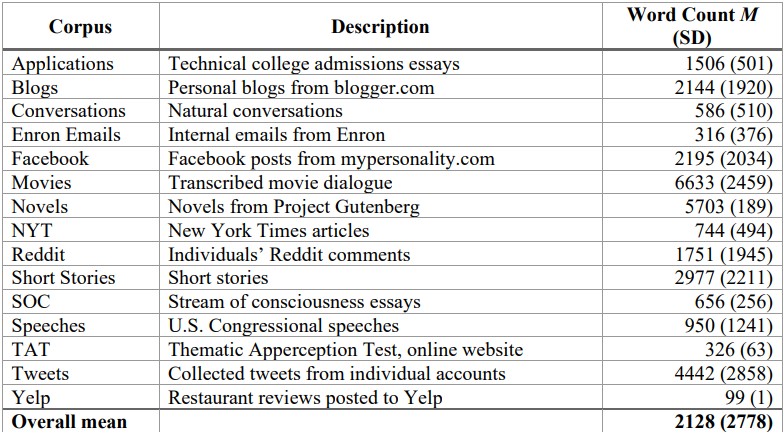
\includegraphics[scale=0.65]{./figures/test-kitchen-corpus.png}
	\caption{The test Kitchen Corpus of 31 Million Words \cite{boyd2022development}}
	\label{FigKitchenCorpus}
\end{figure}

Quantifying the reliability and validity of text analysis tools like LIWC-22 presents challenges different from traditional psychological assessments. Unlike structured questionnaires, natural language doesn't follow repetitive patterns, making it necessary to adjust standards for language-based analyses. This is due to the dynamic nature of verbal behavior in real-world communication, such as social media posts or conversations, where thoughts are expressed and then move on to the next topic.

Evaluating LIWC-22's reliability involves adapting to this non-repetitive nature. For example, the LIWC-22 Anger scale includes 181 words and phrases related to anger. The use of one anger-related word should theoretically correlate with others in the same text. By analyzing these correlations across various texts, LIWC-22 determines internal consistency \cite{boyd2022development}. Validating LIWC's dimensions is complex. While the categories appear relevant, it's crucial to understand how personal and social psychological processes are reflected in language use. For instance, frequent use of words related to "affiliation" may indicate social connections and needs. Determining whether such language use offers insights into someone's social relationships is vital.

LIWC-22 uses Cronbach’s alpha for continuous data and the Kuder–Richardson Formula 20 (KR-20) for binary data to compute reliability metrics \cite{kuder1937theory}. Traditional methods may underestimate reliability due to variable word usage rates. KR-20, however, provides a more accurate measure by considering the binary nature of word presence.

In 2021, over 2,400 studies used LIWC to examine text, combining text analysis with social and psychological behaviors. These studies, including those from LIWC's developers, found correlations between text-detected emotions and self-reported feelings, showing the tool's capability to capture psychological dynamics. Higher correlations were observed when comparing judges' ratings of writing samples with LIWC scores, indicating consistent external validation \cite{boyd2022development}.
\chapter{AI Model for Detecting Depression}

\label{chap:ch4}

\section{Methodology}

\quad In order to develop an accurate AI model for detecting depression from textual data, the choice of the right model and the fine-tuning of its parameters are critical steps. In machine learning, selecting the most appropriate algorithm is very important to the success of any classifying task. This is also true in the case of depression detection, where the complexity and variability of the data demand an approach that is not only accurate but also can work on texts from different cultures. Looking at section 2.2, it was decided to use Random Forest (RF) as the AI model. 

In the context of this study focused on depression detection, the dataset resembles the Breast Cancer Wisconsin dataset (see Section 2.2), because the model is also a binary classifier. However, the model differentiates itself with a higher dimensionality, processing 119 input attributes for the English feature vector dataset and 86 for the Romanian one, which poses a greater complexity in feature representation and selection. For this dataset (Random Forest) RF achieved the highest accuracy at 97.85\%, suggesting it was the most successful in correctly identifying cases of breast cancer. It also had the highest kappa value of 95.03\%. Precision with RF was great as well, hitting a high of 98\%, while its recall was nearly as impressive at 97.9\%, showing its ability to identify most of the positive cases.

For processing the datasets LIWC-22 was used for the original dataset in English and LIWC-2015 for the Romanian translated dataset. This results in the feature vectors that contain numbers associated with each category presented in Figures \ref{LIWC22EnglishDicF1} and \ref{LIWC22EnglishDicF2} for the English 2022 dictionary (119 features), respectively Figures \ref{LIWC2015RomanianDicF1} and \ref{LIWC2015RomanianDicF2} for the Romanian 2015 dictionary (86 features). Except for "Word Count" which represents the number of words in the input text which is a whole number, all the numbers are rational. This comes from the fact that LIWC attributes to a word multiple categories, each with its specific score. Take the word "mad" — it's included in the anger dictionary. Consider "mad" usually shows some level of anger. But sometimes, it means joy ("he’s mad for her") or insanity ("mad as a hatter"). Thankfully, this rarely causes issues because LIWC uses probabilistic language models. If "mad" is used to show positive emotion in a sentence, the writer would typically use other positive words too and fewer anger words. This would give a high positive emotion score and a low anger score.

The resulted feature vectors are then used to train and evaluate the Random Forrest Classifier. There are 3 experiments detailed in the following section. The resulted models are saved and then used to classify the user input in the developed chrome extension. All steps of the proposed approach can be visualized in Figure \ref{proposedApproachFlow}.

\begin{figure}[htbp]
	\centering
		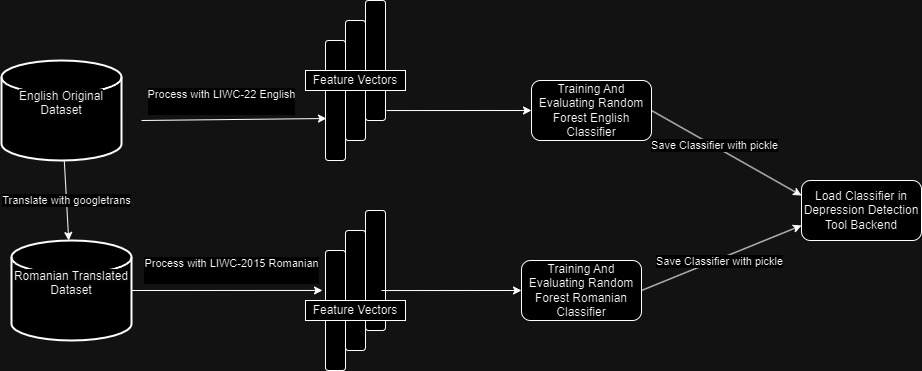
\includegraphics[scale=0.47]{LaTeX Bachelor Thesis Depression Signs Detection/figures/FlowModel.jpg}
	\caption{Proposed Approach Flow}
	\label{proposedApproachFlow}
\end{figure}


\section{Experiments}

\quad To achieve an optimal model, it is essential to explore various training methodologies. This section describes the procedures followed in training the model. There are three experiments: two for the original dataset in English and one for the Romanian translated dataset. The classification flow for them can be visualized in Figure \ref{experimentsFlow}.

\begin{figure}[htbp]
	\centering
		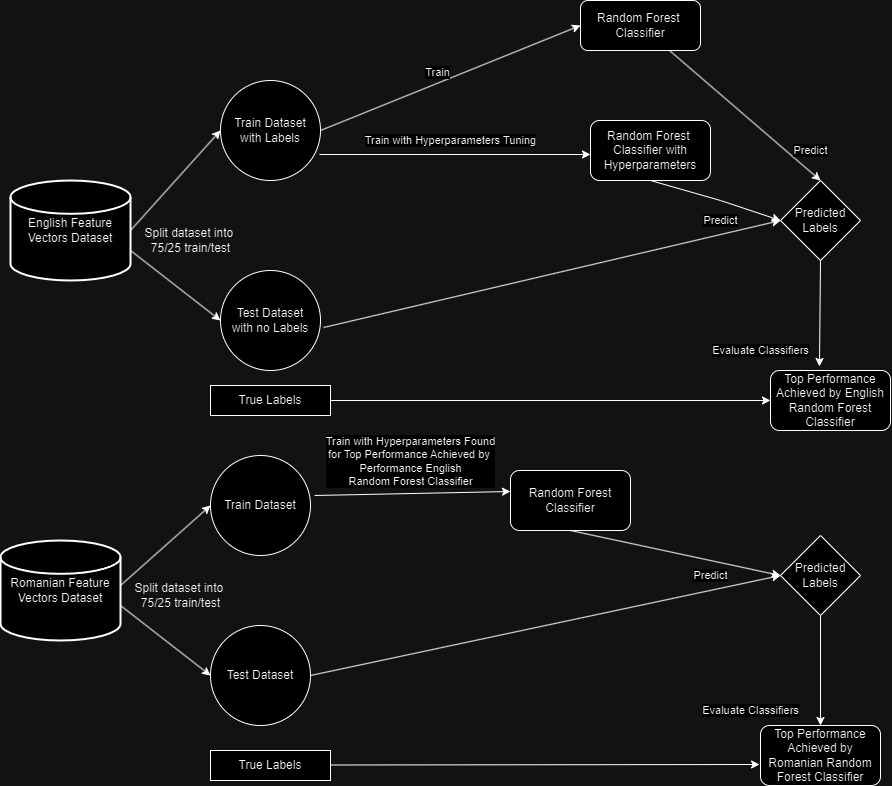
\includegraphics[scale=0.5]{LaTeX Bachelor Thesis Depression Signs Detection/figures/ClassificationFlow.jpg}
	\caption{Experiments Flow}
	\label{experimentsFlow}
\end{figure}

\subsection{First Experiment for English Language}

\quad In the initial training experiment, all available features were utilized without any adjustments to hyperparameters. The default settings of the Random Forest Classifier from sklearn were applied \cite{sklearn_api}. The dataset was partitioned in a 75/25 train/test split, ensuring an equal distribution of positive and negative cases by using the stratify option, as illustrated in Figure \ref{codeTrainRF}.

\begin{figure}[htbp]
	\centering
		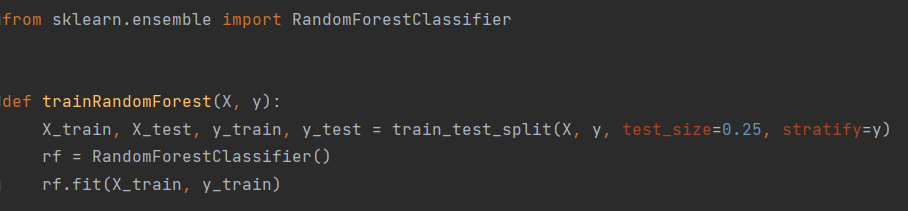
\includegraphics[scale=0.6]{LaTeX Bachelor Thesis Depression Signs Detection/figures/codeTrainingRF.png}
	\caption{Python code used for the initial training of the Random Forest Classifier}
	\label{codeTrainRF}
\end{figure}

The first experiment's results reveal a strong performance across the chosen metrics. The Classification Metrics plot shows high values for Accuracy (0.96), Precision (0.99), Recall (0.93), and F1 Score (0.96), indicating an efficient model with a balanced approach to both relevance (precision) and completeness (recall) \ref{classificationMetricsFirstExperiment}.

\begin{figure}[htbp]
	\centering
		\includegraphics[scale=0.8]{LaTeX Bachelor Thesis Depression Signs Detection/figures/metrics/experiment1English/classificationMetrics.jpg}
	\caption{Classification Metrics First Experiment}
	\label{classificationMetricsFirstExperiment}
\end{figure}

The Confusion Matrix provides a visual confirmation of the model's performance, with a high number of true positives (891) and true negatives (969), and relatively few false positives (6) and false negatives (67) \ref{confusionMatrixFirstExperiment}. This suggests the model has more problems when finding depression.

\begin{figure}[htbp]
	\centering
		\includegraphics[scale=0.8]{LaTeX Bachelor Thesis Depression Signs Detection/figures/metrics/experiment1English/confusionMatrix.jpg}
	\caption{Confusion Matrix First Experiment}
	\label{confusionMatrixFirstExperiment}
\end{figure}

Looking at the ROC Curve, the model demonstrates an excellent ability to distinguish between the classes, as evidenced by the area under the curve (AUC) being close to 1 (0.99) \ref{rocCurveFirstExperiment}. This suggests that the model has a good discrimination capability with a high true positive rate and a low false positive rate across different thresholds.

\begin{figure}[htbp]
	\centering
		\includegraphics[scale=0.8]{LaTeX Bachelor Thesis Depression Signs Detection/figures/metrics/experiment1English/roc_curve.jpg}
	\caption{ROC Curve First Experiment}
	\label{rocCurveFirstExperiment}
\end{figure}

The Top 10 Feature Importances plot indicates which features have the most influence on the model's predictions. The leading features, labeled as 'WC' (Word Count) and 'WPS' (Words per Sentence), seem to be the most significant drivers, with the others contributing to varying lesser degrees \ref{top10FeaturesFirstExperiment}. This shows us that the length of the given text is very important in order for the model to give an accurate prediction.

\begin{figure}[htbp]
	\centering
		\includegraphics[scale=0.5]{LaTeX Bachelor Thesis Depression Signs Detection/figures/metrics/experiment1English/top10features.jpg}
	\caption{Top 10 Feature Importances First Experiment}
	\label{top10FeaturesFirstExperiment}
\end{figure}

Overall, the model appears to be highly effective, with strong performance indicators, which seems to be the result of the analysis done for choosing the pre-processing methods and classifier, namely LIWC \cite{boyd2022development} and Random Forrest.

\subsection{Second Experiment for English Language}
The selection of Random Forest hyperparameters is guided by the study \cite{probst2019hyperparameters}. The adjusted hyperparameters are:

\begin{itemize}
  \item \textbf{mtry}: This represents the number of features considered for splitting at each node. Lower values promote tree diversity and are beneficial when there are many relevant predictors. Given the large feature set, a value lower than the default square root of the number of features is suggested to prevent dominant features from overshadowing others.
  \item \textbf{Number of Trees}: A sufficient number of trees ensures stable predictions and importance estimates. While more trees generally improve model performance, beyond a certain point the marginal gains diminish. For practical purposes, between 500 to 1000 trees are recommended.
  \item \textbf{Node Size}: The node size controls the depth of the tree. Smaller node sizes can potentially lead to over-fitting, particularly when the number of features is high. A larger than 1 node size is preferred to mitigate this risk and improve computational efficiency.
  \item \textbf{Sample Size}: The proportion of data used for training each tree. Smaller sample sizes lead to more diversity but can decrease individual tree accuracy. Optimal sample size needs to be problem-specific but sampling a subset, such as between 20\% and 90\% of the data, can yield good results while reducing runtime. 
\end{itemize}

These hyperparameters were tuned using Sequential Model-Based Optimization (SMBO) to determine their optimal values while considering the Area Under the ROC Curve (AUC) as the performance metric \cite{probst2019hyperparameters}.

For the depression binary classifier multiple configurations were tested. It was noticed that the optimal ranges for the hyperparameters were:
\begin{itemize}
    \item \textbf{mtry}: between 6 and 10
    \item \textbf{Number of trees}: between 700 and 1000
    \item \textbf{Node Size}: between 3 and 9
    \item \textbf{Sample size}: between 6 and 9
\end{itemize}

After training with all combinations of the mentioned ranges, the one who got the best results was 6 for mtry, 900 for number of trees, 3 for node size and 8 for sample size. The same metrics as in the first experiment were used to analyze the performance of the model and improvements were seen. For the classification metrics accuracy(0.97) has improved by 0.01, precision stayed the same, recall(0.96) was the one who improved the most by 0.03, and F1-score(0.97) improved by 0.01. These values can be seen comparing Figure \ref{classificationMetricsFirstExperiment}, which shows the classification metrics for the first experiment, with Figure \ref{classificationMetricsSecondExperiment}, which shows them for the second experiment. This shows that because of hyperparameters tuning, it succeeded in improving the part where the model from the first experiment lacked.

\begin{figure}[htbp]
	\centering
		\includegraphics[scale=0.8]{LaTeX Bachelor Thesis Depression Signs Detection/figures/metrics/experiment2English/classificationMetrics.jpg}
	\caption{Classification Metrics Second Experiment}
	\label{classificationMetricsSecondExperiment}
\end{figure}

In the case of the confusion matrix for the second experiment \ref{confusionMatriSecondExperiment} it can be discovered that in comparison with the one for the first experiment \ref{confusionMatrixFirstExperiment}, as can the improvement of recall also tell, the values of the false positives decreased, from 67 to 43.

\begin{figure}[htbp]
	\centering
		\includegraphics[scale=0.8]{LaTeX Bachelor Thesis Depression Signs Detection/figures/metrics/experiment2English/confusionMatrix.jpg}
	\caption{Confusion Matrix Second Experiment}
	\label{confusionMatriSecondExperiment}
\end{figure}

For the ROC curve for this experiment \ref{rocCurveSecondExperiment}, the area stayed the same when looking to the first two digits, but an improvement of the true positive rate can be noticed from the initial experiment \ref{rocCurveFirstExperiment}.

\begin{figure}[htbp]
	\centering
		\includegraphics[scale=0.8]{LaTeX Bachelor Thesis Depression Signs Detection/figures/metrics/experiment2English/roc_curve.jpg}
	\caption{ROC Curve Second Experiment}
	\label{rocCurveSecondExperiment}
\end{figure}

Seeing the top 10 features of the second experiment \ref{top10FeaturesSecondExperiment}, it was noticed that in comparison with the initial one \ref{top10FeaturesFirstExperiment} that even though WC (Word Count) and WS (Words per Sentence) are the still the most important features, they are now by much less, from 0.12 and 0.10 to both being at 0.09. This shows that now there are more features taken into account when the model makes the classification and each is more influential. Also it is remarked that a feature in the first ten was changed, namely emo\_anx (anxiety) with cause (causation).

\begin{figure}[htbp]
	\centering
		\includegraphics[scale=0.5]{LaTeX Bachelor Thesis Depression Signs Detection/figures/metrics/experiment2English/top10features.jpg}
	\caption{Top 10 Feature Importances Second Experiment}
	\label{top10FeaturesSecondExperiment}
\end{figure}

\subsection{Experiment for Romanian Language}

\quad For the Romanian language model, the methodology was replicated consistently. LIWC served as the tool for preprocessing the data. However, the most recent English dictionary for LIWC-22 has not been translated into Romanian. The latest available version for Romanian is the LIWC-2015 dictionary, which contains only 86 features, compared to the 119 features available in the English version.

The training approach was aligned with the methodology used for the English model during the second experiment. The hyperparameters and the proportion of training to testing data remain consistent:

\begin{itemize}
\item \textbf{train/test split}: Maintained at 75/25, using stratification based on the 'is\_depression' label
\item \textbf{mtry}: 6
\item \textbf{Number of trees}: 900
\item \textbf{Node Size}: 3
\item \textbf{Sample size}: 8
\end{itemize}

This methodology facilitates a direct comparison between the performance of the Romanian and English models, ensuring consistent evaluation criteria across both. The same metrics were used for analysis. In terms of classification metrics, the most notable discrepancy arises in recall, where the Romanian model scores 0.87, falling short of the English model's 0.96 by 9 percentage points. Additionally, both accuracy and the F1-score have diminished by 0.05, while precision experienced the least impact, decreasing from 0.99 to 0.97. These metrics are illustrated in Figure \ref{classificationMetricsSecondExperiment} for the English model and in Figure \ref{classificationMetricsRomanianExperiment} for the Romanian model.

The diminished recall in the Romanian model suggests it is less adept at identifying true positive cases as compared to the English model. This lower performance may come from the nuances lost during the translation of the dataset from English to Romanian using the Googletrans library \cite{googletranslib}. Such translation challenges could contribute to the model’s reduced effectiveness, highlighting the influence of linguistic or cultural differences on the model’s ability to generalize across languages. The smaller reductions in accuracy and F1-score indicate that while the model is somewhat less effective overall, it still maintains a reasonable level of precision.

\begin{figure}[htbp]
	\centering
		\includegraphics[scale=0.8]{LaTeX Bachelor Thesis Depression Signs Detection/figures/metrics/experimentRomanian/classificationMetrics.jpg}
	\caption{Classification Metrics Romanian Model}
	\label{classificationMetricsRomanianExperiment}
\end{figure}

The confusion matrix \ref{confusionMatrixRomanianExperiment} illustrates a significant increase in false positives, rising from 43 in the English model \ref{confusionMatriSecondExperiment} to 123 in the Romanian model. However, the rise in false negatives was less marked, increasing from 7 to 26.

\begin{figure}[htbp]
	\centering
		\includegraphics[scale=0.8]{LaTeX Bachelor Thesis Depression Signs Detection/figures/metrics/experimentRomanian/confusionMatrix.jpg}
	\caption{Confusion Matrix Romanian Model}
	\label{confusionMatrixRomanianExperiment}
\end{figure}

Regarding the ROC curve, the Area Under the Curve (AUC) experienced a slight decrease of 0.01, as depicted in Figure \ref{rocCurveRomanianExperiment} compared to Figure \ref{rocCurveSecondExperiment}. These metrics collectively indicate that the issues observed during the experimentation with the English model are more pronounced in the Romanian classifier.

\begin{figure}[htbp]
	\centering
		\includegraphics[scale=0.8]{LaTeX Bachelor Thesis Depression Signs Detection/figures/metrics/experimentRomanian/roc_curve.jpg}
	\caption{ROC Curve Romanian Model}
	\label{rocCurveRomanianExperiment}
\end{figure}

The most significant features for the Romanian classifier \ref{top10FeaturesRomanianExperiment} align more closely with those observed in the initial experiment for the English model \ref{top10FeaturesFirstExperiment}. Notably, Word Count (WC) has risen above 0.12, surpassing the prominence it held in the first experiment. This contrasts with the enhancements seen in the second English experiment \ref{top10FeaturesSecondExperiment}, where a diminished reliance on WC and WPS (Words per Sentence) indicated a broader array of features influencing the English classifier’s decisions. However, this diversification does not appear to extend to the Romanian model.

Some features remain consistent with the English LIWC-22 dictionary features listed in the top 10 for the second experiment; for instance, "sad" aligns with "emo\_sad", and both "cause" and "health" are both present and "negemo" is the same as "emo\_neg". The "anx" feature mirrors "emo\_anx" from the first experiment’s top features. The presence of "Period" suggests that the Googletrans library has introduced punctuation marks, which have become a significant element. The evolution from LIWC-2015 to LIWC-22 is further evidenced by the removal of the "interrog" category in the Romanian model’s top 10 features, which was dropped in LIWC-22 due to its low base rates, internal reliability, or infrequent usage, as noted in \cite{boyd2022development}. The "ipron" feature might also result from the machine translation process.

\begin{figure}[htbp]
	\centering
		\includegraphics[scale=0.5]{LaTeX Bachelor Thesis Depression Signs Detection/figures/metrics/experimentRomanian/top10features.jpg}
	\caption{Top 10 Features Romanian Model}
	\label{top10FeaturesRomanianExperiment}
\end{figure}



\chapter{Implementation Details}
\label{chap:ch5}

\quad This chapter details the architecture used, detailing the design, and discussing the implementation specifics.

\section{Architechure}

\quad The tool is a web application, specifically a Chrome extension, named "Depression Signs Detector" and has the icon showed in Figure \ref{depressionsSignsDetectorIcon}, which has a minimalist design showing a heart which has as the left part a brain, showing the importance of mental health. The developed tool's backend operates locally, and the frontend is configured in developer mode as a Chrome extension.

It adheres to the REST software architectural design. RESTful Web Services facilitate communication with the client through the receipt of HTTP methods such as GET, POST, PUT, DELETE, accompanied by some additional data, and respond with the precise data needed for the client to display information to the user. The response format is typically JSON (JavaScript Object Notation), although XML is also possible. This web application is divided into two main servers: the frontend and the backend.

\begin{figure}[htbp]
	\centering
		
\includegraphics[scale=0.1]{LaTeX Bachelor Thesis Depression Signs Detection/figures/icon1024.png}
	\caption{Depression Signs Detector Icon}
	\label{depressionsSignsDetectorIcon}
\end{figure}

\section{Backend}

\quad The backend serves as the data access layer of an application. Typically, it accesses the database to fetch data and carries out various computations with this data. However, in this specific application, there is no database layer since there is no requirement for data storage. Here, the backend is facilitated by a Python webserver, constructed using Flask. Flask is recognized as a lightweight micro web application framework for Python \cite{ronacher2021flask}, selected for its straightforward configuration and the freedom it offers in architectural choices, such as the absence of a database. Unlike more comprehensive Python web frameworks like Django, Flask does not provide a database abstraction layer, form validation, or other extensive libraries. The choice of Flask over other frameworks was influenced by the simplicity it brings to server management.

\begin{figure}[htbp]
	\centering
		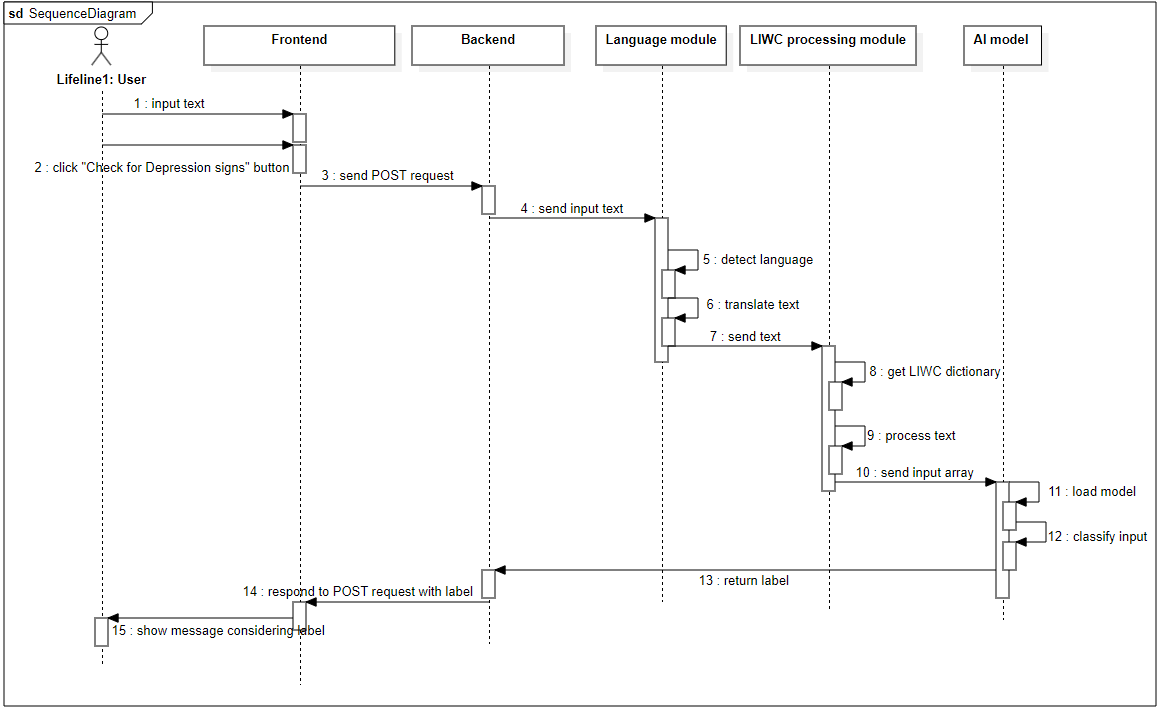
\includegraphics[scale=0.5]{LaTeX Bachelor Thesis Depression Signs Detection/figures/SequnceDiagram.png}
	\caption{Sequence Diagram for Detecting Signs of Depression}
	\label{seqDiag}
\end{figure}

The only role of the backend in this application is to handle a POST request which is annotated with "/classify" containing the input text in its body, and to respond with a 1 if the AI model determines that the text is indicative of a depressed individual, and a 0 otherwise. Firstly the input text in the body of the POST request, used for security reasons instead of GET, is checked in the Language module, showed in Figure \ref{seqDiag}. With the help of googlelib \cite{googletranslib}, which also has a detect language functionality, it is seen whether the received text is in Romanian or English. If not, we translate it into English.

Considering the language the text is in after the language module, an LIWC dictionary is selected, namely for English "LIWC-22" and for Romanian "Ro-LIWC-2015". Then, the text is processed in python with the help of the CLI provided by LIWC and the output is received in cmd as seen in Figure \ref{codeLiwcCli}.

\begin{figure}[htbp]
	\centering
		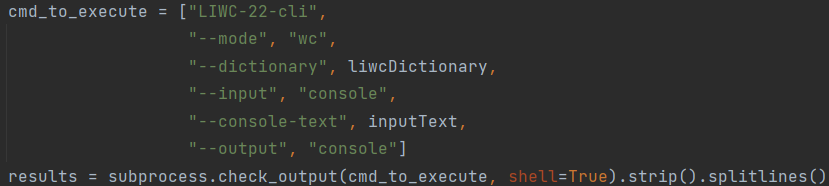
\includegraphics[scale=0.5]{LaTeX Bachelor Thesis Depression Signs Detection/figures/codeLiwcCLI.png}
	\caption{Python Code to Process Text Using LIWC CLI }
	\label{codeLiwcCli}
\end{figure}

Once more, based on the language of the text, the appropriate AI model, either Romanian or English, is loaded. This model is then used to classify the text, and the label is sent back to the frontend, illustrated in Figure \ref{seqDiag}.

\section{Frontend}

\quad The frontend of this application is developed using the React JavaScript library and TypeScript. As seen in the Figure \ref{interface}, it containts a text box where the text to be classified is to be put and a button for initiating the POST request. After receiving the response from backend containing the label predicted by the classifier, two messages can be shown:
\begin{itemize}
    \item label 0 (no depression detected): It appears there are no signs of depression, which is reassuring. Thank you for taking the time to look out for the well-being of the person who wrote this message.
    \item label 1 (depression detected):  Signs of depression detected. It might be helpful to reach out and talk more with the person who wrote this message. Offering a listening ear can make a big difference.
\end{itemize}

\begin{figure}[htbp]
	\centering
		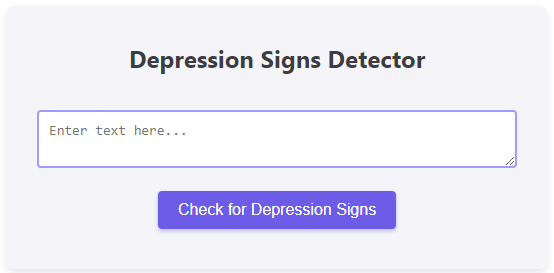
\includegraphics[scale=0.5]{LaTeX Bachelor Thesis Depression Signs Detection/figures/interface.png}
	\caption{Chrome Extension User Interface}
	\label{interface}
\end{figure}









\chapter{Conclusions and Future Work}
\label{conclusions}

\quad Developing a multilingual tool presents significant challenges. There is a much richer body of literature for English than for Romanian, which impacts the performance of AI models, as evidenced by our experiments. The English model achieved a precision of 96\%, significantly higher than the Romanian model's 87\%. This difference largely comes from the translation methods used and the limitations of the pre-processing tool LIWC. Despite using Google Translate, a leading translation service, the Googlelib \cite{googletranslib} encountered difficulties in maintaining the original text's meaning. Additionally, the most recent version of LIWC, LIWC-22, is only available in English, which meant a downgrade to LIWC-2015 for Romanian, which is seven years behind in advancements, as reflected in the precision of our Romanian classifier.

For future improvements, employing an AI-based translation tool could preserve text meaning more effectively. Also, since LIWC \cite{boyd2022development} specifies its use strictly for academic purposes, any commercial application would need to adopt a different pre-processing approach to cover licensing costs. Such advancements could greatly aid in targeted marketing for psychologists or enhancing mental health awareness, aligning with the goals of the "Depression Signs Detector" tool. The next step for the tool is its deployment to a production environment, transitioning from localhost to a cloud hosting platform to ensure broader accessibility and reliability.

As a computer science researcher, I cannot provide human-based validation for diagnosing depression, such validation must be performed by a specialist. Unlike object detection in images, which can be visually verified by nearly anyone, assessing the accuracy of depression detection outputs is beyond a programmer’s capability.

Moreover, while communicating, words represent only a minor fraction of the information conveyed. The tool, which solely analyzes text, is insufficient to conclusively determine if a person is depressed. Therefore, it is important to note that the tool serves merely as a preliminary assessment of a person’s emotional state, a thorough evaluation requires a professional in psychology. For a more accurate computer-based analysis, it would be necessary to consider all aspects of communication, both verbal and nonverbal.


%\addcontentsline{toc}{chapter}{Concluzii}
%\addcontentsline{toc}{chapter}{Conclusions}

\bibliography{references}

\end{document}
%TODO: cand cumpar licenta pt liwc schimbat inloc de 64 input attributes cu cate o sa am